\chapter{Code Generation}

This chapter describes the code generation process. The examples of
generated code presented here are produced by the compiler, but some
cosmetic changes have been made to enhance readability.

Code generation is done one procedure at a time. An Icon procedure is,
in general, translated into several C functions. There is always an
\textit{outer function}
for the procedure. This is the function that is seen as implementing
the procedure. In addition to the outer function, there may be several
functions for success continuations that are used to implement
generative expressions.

The outer function of a procedure must have features that support the
semantics of an Icon call, just as a function implementing a run-time
operation does. In general, a procedure must have a procedure block at
run time. This procedure block references the outer function. All
functions referenced through a procedure block must conform to the
compiler system's standard calling conventions. However, invocation
optimizations usually eliminate the need for procedure variables and
their associated procedure blocks. When this happens, the calling
conventions for the outer function can be tailored to the needs of the
procedure.

As explained in Chapter 14, the standard calling convention requires
four parameters: the number of arguments, a pointer to the beginning
of an array of descriptors holding the arguments, a pointer to a
result location, and a success continuation to use for suspension. The
function itself is responsible for dereferencing and argument list
adjustment.  In a tailored calling convention for an outer function of
a procedure, any dereferencing and argument list adjustment is done at
the call site. This includes creating an Icon list for the end of a
variable-sized argument list. The compiler produces code to do this
that is optimized to the particular call. An example of an
optimization is eliminating dereferencing when type inferencing
determines that an argument cannot be a variable reference.

The number of arguments is never needed in these tailored calling
conventions because the number is fixed for the procedure. Arguments
are still passed via a pointer to an array of descriptors, but if
there are no arguments, no pointer is needed. If the procedure returns
no value, no result location is needed. If the procedure does not
suspend, no success continuation is needed.

In addition to providing a calling interface for the rest of the
program, the outer function must provide local variables for use by
the code generated for the procedure. These variables, along with
several other items, are located in a procedure frame. An Icon
procedure frame is implemented as a C structure embedded within the
frame of its outer C function (that is, as a local struct
definition). Code within the outer function can access the procedure
frame directly. However, continuations must use a pointer to the
frame. A global C variable, \texttt{pfp}, points to the frame of the currently
executing procedure. For efficiency, continuations load this pointer
into a local register variable. The frame for a main procedure might
have the following declaration.

\goodbreak
\begin{iconcode}
struct PF00\_main \{\\
\>struct p\_frame old\_pfp;\\
\>dptr old\_argp;\\
\>dptr rslt;\\
\>continuation succ\_cont;\\
\>struct \{\\
\>\>struct tend\_desc *previous;\\
\>\>int num;\\
\>\>struct descrip d[5];\\
\>\>\} tend;\\
\>\};\\
\end{iconcode}

\noindent with the definition

\iconline{ \>struct PF00\_main frame; }

\noindent in the procedure's outer function. A procedure frame always
contains the following five items: a pointer to the frame of the
caller, a pointer to the argument list of the caller, a pointer to the
result location of this call, a pointer to the success continuation of
this call, and an array of tended descriptors for this procedure. It
may also contain C integer variables, C double variables, and string
and cset buffers for use in converting values. If debugging is
enabled, additional information is stored in the frame. The structure
\texttt{p\_frame} is a generic procedure frame containing a single
tended descriptor. It is used to define the pointer \texttt{old\_pfp}
because the caller can be any procedure.

The argument pointer, result location, and success continuation of the
call must be available to the success continuations of the
procedure. A global C variable, \texttt{argp}, points the argument list for the
current call. This current argument list pointer could have been put
in the procedure frame, but it is desirable to have quick access to
it. Quick access to the result location and the success continuation
of the call is less important, so they are accessed indirectly through
the procedure frame.

The array of descriptors is linked onto the chain used by the garbage
collector to locate tended descriptors. These descriptors are used for
Icon variables local to the procedure and for temporary variables that
hold intermediate results. If the function is responsible for
dereferencing and argument list adjustment (that is, if it does not
have a tailored calling convention), the modified argument list is
constructed in a section of these descriptors.

The final thing provided by the outer function is a \textit{control
environment} in which code generation starts. In particular, it
provides the bounding environment for the body of the procedure and
the implicit failure at the end of the procedure. The following C
function is the tailored outer function for a procedure named
\texttt{p}. The procedure has arguments and returns a result. However,
it does not suspend, so it needs no success continuation.

\goodbreak
\begin{iconcode}
static int P01\_p(args, rslt)\\
dptr args;\\
dptr rslt;\\
\{\\
\>struct PF01\_p frame;\\
\>register int signal;\\
\>int i;\\
\>frame.old\_pfp = pfp;\\
\>pfp = (struct p\_frame )\&frame;\\
\>frame.old\_argp = argp;\\
\>frame.rslt = rslt;\\
\>frame.succ\_cont = NULL;\\
\\
\>for (i = 0; i < 3; ++i)\\
\>\>frame.tend.d[i].dword = D\_Null;\\
\>argp = args;\\
\>frame.tend.num = 3;\\
\>frame.tend.previous = tend;\\
\>tend = (struct tend\_desc )\&frame.tend;\\
\\
\>\textit{translation of the body of procedure p}\\
\\
L10: /* bound */\\
L4: /* proc fail */\\
\>tend = frame.tend.previous;\\
\>pfp = frame.old\_pfp;\\
\>argp = frame.old\_argp;\\
\>return A\_Resume;\\
L8: /* proc return */\\
\>tend = frame.tend.previous;\\
\>pfp = frame.old\_pfp;\\
\>argp = frame.old\_argp;\\
\>return A\_Continue;\\
\>\}\\
\end{iconcode}

\noindent
The initialization code reflects the fact that this function has three
tended descriptors to use for local variables and intermediate
results. \texttt{L10} is both the bounding label and the failure label for the
body of the procedure. Code to handle procedure failure and return
(except for setting the result value) is at the end of the outer
function. As with bounding labels, the labels for these pieces of code
have associated signals. If a procedure fail or return occurs in a
success continuation, the continuation returns the corresponding
signal which is propagated to the outer function where it is converted
into a goto. The code for procedure failure is located after the body
of the procedure, automatically implementing the implicit failure at
the end of the procedure.


\section{Translating Icon Expressions}

Icon's goal-directed evaluation makes the implementation of control
flow an important issue during code generation. Code for an expression
is generated while walking the expression's syntax tree in forward
execution order. During code generation there is always a
\textit{current failure action}. This action is either ``branch to a
label'' or ``return a signal''.  When the translation of a procedure
starts, the failure action is to branch to the bounding label of the
procedure body. The action is changed when generators are encountered
or while control structures that use failure are being translated.

The allocation of temporary variables to intermediate results is
discussed in more detail later. However, some aspects of it will be
addressed before presenting examples of generated code. The result
location of a subexpression may be determined when the parent
operation is encountered on the way down the syntax tree. This is
usually a temporary variable, but does not have to be. If no location
has been assigned by the time the code generator needs to use it, a
temporary variable is allocated for it. This temporary variable is
used in the code for the parent operation.

The code generation process is illustrated below with examples that
use a number of control structures and operations.  Code generation
for other features of the language is similar.

Consider the process of translating the following Icon expression: 

\iconline{return if a = (1 | 2) then "yes" else "no" }

\noindent
When this expression is encountered, there is some current failure
action, perhaps a branch to a bounding label. The \texttt{return}
expression produces no value, so whether a result location has been
assigned to it is of no consequence. If the argument of a
\texttt{return} fails, the procedure fails. To handle this
possibility, the current failure action is set to branch to the label
for procedure failure before translating the argument (in this
example, that action is not used).  The code for the argument is then
generated with its result location set to the result location of the
procedure itself. Finally the result location is dereferenced and
control is transferred to the procedure return label. The
dereferencing function, \texttt{deref}, takes two arguments: a pointer
to a source descriptor and a pointer to a destination descriptor.

\goodbreak
\begin{iconcode}
\>\>\textit{code for the if expression }\\
\>\>deref(rslt, rslt);\\
\>\>goto L7 /* proc return */;\\
\end{iconcode}


The control clause of the \texttt{if} expression must be bounded. The
code implementing the \texttt{then} clause must be generated following
the bounding label for the control clause. A label must also be set up
for the \texttt{else} clause with a branch to this label used as the
failure action for the control clause. Note that the result location
of each branch is the result location of the \texttt{if} expression
which is in turn the result location of the procedure. Because neither
branch of the \texttt{if} expression contains operations that suspend,
the two control paths can be brought together with a branch to a
label.

\goodbreak
\begin{iconcode}
\>\>\textit{code for control clause}\\
\>L4: /* bound */\\
\>\>rslt->vword.sptr = "yes";\\
\>\>rslt->dword = 3;\\
\>\>goto L6 /* end if */;\\
\>L5: /* else */\\
\>\>rslt->vword.sptr = "no";\\
\>\>rslt->dword = 2;\\
\>L6: /* end if */\\
\end{iconcode}

\noindent
Using a branch and a label to bring together the two control paths of
the \texttt{if} expression is an optimization. If the \texttt{then} or
the \texttt{else} clauses contain operations that suspend, the general
continuation model must be used. In this model, the code following the
\texttt{if} expression is put in a success continuation, which is then
called at the end of both the code for the \texttt{then} clause and
the code for the \texttt{else} clause.

Next consider the translation of the control clause. The numeric
comparison operator takes two operands. In this translation, the
standard calling conventions are used for the library routine
implementing the operator. Therefore, the operands must be in an array
of descriptors. This array is allocated as a sub-array of the tended
descriptors for the procedure. In this example, tended location 0 is
occupied by the local variable, \texttt{a}. Tended locations 1 and 2 are free
to be allocated as the arguments to the comparison operator. The code
for the first operand simply builds a variable reference.

\goodbreak
\begin{iconcode}
\>frame.tend.d[1].dword = D\_Var;\\
\>frame.tend.d[1].vword.descptr = \&frame.tend.d[0] /* a */;\\
\end{iconcode}

\noindent
However, the second operand is alternation. This is a generator and
requires a success continuation. In this example, the continuation is
given the name \texttt{P02\_main} (the Icon expression is part of the main
procedure). The continuation contains the invocation of the run-time
function implementing the comparison operator and the end of the
bounded expression for the control clause of the \texttt{if}. The function
\texttt{O0o\_numeq} implements the comparison operator. The \texttt{if} expression
discards the operator's result. This is accomplished by using the
variable \texttt{trashcan} as the result location for the call. The compiler
knows that this operation does not suspend, so it passes a null
continuation to the function. The end of the bounded expression
consists of a transfer of control to the bounding label. This is
accomplished by returning a signal. The continuation is

\goodbreak
\begin{iconcode}
static int P02\_main()\\
\{\\
register struct PF00\_main *rpfp;\\

rpfp = (struct PF00\_main *)pfp;\\
switch (O0o\_numeq(2, \&(rpfp->tend.d[1]), \&trashcan, (continuation)NULL))\\
\>\{\\
\>case A\_Continue:\\
\>\>break;\\
\>case A\_Resume:\\
\>\>return A\_Resume;\\
\>\}\\
\ return 4; /* bound */\\
\}\\
\end{iconcode}

\noindent
Each alternative of the alternation must compute the value of its
subexpression and call the success continuation. The failure action
for the first alternative is to branch to the second alternative. The
failure action of the second alternative is the failure action of the
entire alternation expression. In this example, the failure action is
to branch to the \texttt{else} label of the \texttt{if} expression. In
each alterative, a bounding signal from the continuation must be
converted into a branch to the bounding label. Note that this bounding
signal indicates that the control expression succeeded.

\goodbreak
\begin{iconcode}
frame.tend.d[2].dword = D\_Integer;\\
frame.tend.d[2].vword.integr = 1;\\
switch (P02\_main()) \{\\
\>case A\_Resume:\\
\>\>goto L2 /* alt */;\\
\>case 4 /* bound */:\\
\>\>goto L4 /* bound */;\\
\>\}\\
L2: /* alt */\\
\>frame.tend.d[2].dword = D\_Integer;\\
\>frame.tend.d[2].vword.integr = 2;\\
\>switch (P02\_main()) \{\\
\>\>case A\_Resume:\\
\>\>\>goto L5 /* else */;\\
\>\>case 4 /* bound */:\\
\>\>\>goto L4 /* bound */;\\
\>\>\}\\
\end{iconcode}


The code for the entire \texttt{return} expression is obtained by putting
together all the pieces. The result is the following code (the code
for \texttt{P02\_main} is not repeated).

\goodbreak
\begin{iconcode}
frame.tend.d[1].dword = D\_Var;\\
frame.tend.d[1].vword.descptr = \&frame.tend.d[0] /* a */;\\
frame.tend.d[2].dword = D\_Integer;\\
frame.tend.d[2].vword.integr = 1;\\
switch (P02\_main()) \{\\
\>case A\_Resume:\\
\>\>goto L2 /* alt */;\\
\>case 4 /* bound */:\\
\>\>goto L4 /* bound */;\\
\>\}\\
L2: /* alt */\\
\>frame.tend.d[2].dword = D\_Integer;\\
\>frame.tend.d[2].vword.integr = 2;\\
\>switch (P02\_main()) \{\\
\>\>case A\_Resume:\\
\>\>\>goto L5 /* else */;\\
\>\>case 4 /* bound */:\\
\>\>\>goto L4 /* bound */;\\
\>\>\}\\
L4: /* bound */\\
\>rslt->vword.sptr = yes;\\
\>rslt->dword = 3;\\
\>goto L6 /* end if */;\\

L5: /* else */\\
\>rslt->vword.sptr = no;\\
\>rslt->dword = 2;\\
L6: /* end if */\\
\>deref(rslt, rslt);\\
\>goto L7 /* proc return */;\\
\end{iconcode}


\section{Signal Handling}

In order to produce signal handling code, the code generator must know
what signals may be returned from a call. These signals may be either
directly produced by the operation (or procedure) being called or they
may originate from a success continuation. Note that either the
operation or the continuation may be missing from a call, but not
both. The signals produced directly by an operation are
\texttt{A\_Resume}, \texttt{A\_Continue}, and \texttt{A\_FallThru}
(this last signal is only used internally within in-line code).

The signals produced by a success continuation belong to one of three
categories: \texttt{A\_Resume}, signals corresponding to labels within the
procedure the continuation belongs to, and signals corresponding to
labels in procedures farther down in the call chain. The last category
only occurs when the procedure suspends. The success continuation for
the procedure call may return a signal belonging to the calling
procedure. This is demonstrated in the following example (the
generated code has been ``cleaned-up'' a little to make it easier to
follow).  The Icon program being translated is

\goodbreak
\begin{iconcode}
procedure main()\\
\>write(p())\\
end\\
procedure p()\\
\>suspend 1 to 10\\
end\\
\end{iconcode}


The generative procedure \texttt{p} is called in a bounded context. The code
generated for the call is

\goodbreak
\begin{iconcode}
switch (P01\_p(\&frame.tend.d[0], P05\_main)) \{\\
\>case 7 /* bound */:\\
\>\>goto L7 /* bound */;\\
\>case A\_Resume:\\
\>\>goto L7 /* bound */;\\
\>\}\\
L7: /* bound */\\
\end{iconcode}

\noindent
This call uses the following success continuation. The continuation
writes the result of the call to \texttt{p} then signals the end of the bounded
expression.

\goodbreak
\begin{iconcode}
static int P05\_main() \{\\
\>register struct PF00\_main *rpfp;\\
\\
\>rpfp = (struct PF00\_main )pfp;\\
\>F0c\_write(1, \&rpfp->tend.d[0], \&trashcan, (continuation)NULL);\\
\>return 7; /* bound */\\
\}\\
\end{iconcode}

\noindent
The \texttt{to} operator in procedure \texttt{p} needs a success
continuation that implements procedure suspension. Suspension is
implemented by switching to the old procedure frame pointer and old
argument pointer, then calling the success continuation for the call
to \texttt{p}. The success continuation is accessed with the
expression \texttt{rpfp--{\textgreater}succ\_cont}.  In this example,
the continuation will only be the \texttt{function P05\_main}. The
suspend must check the signal returned by the procedure call's success
continuation. However, the code generator does not try to determine
exactly what signals might be returned by a continuation belonging to
another procedure. Such a continuation may return an
\texttt{A\_Resume} signal or a signal belonging to some procedure
farther down in the call chain. In this example, bounding signal 7
will be returned and it belongs to \texttt{main}.

If the call's success continuation returns \texttt{A\_Resume}, the procedure
frame pointer and argument pointer must be restored, and the current
failure action must be executed. In this case, that action is to
return an \texttt{A\_Resume} signal to the \texttt{to} operator. If the call's success
continuation returns any other signal, that signal must be propagated
back through the procedure call. The following function is the success
continuation for the \texttt{to} operator.

\goodbreak
\begin{iconcode}
static int P03\_p()\\
\{\\
\>register int signal;\\
\>register struct PF01\_p *rpfp;\\
\\
\>rpfp = (struct PF01\_p *)pfp;\\
\>deref(rpfp->rslt, rpfp->rslt);\\
\>pfp = rpfp->old\_pfp;\\
\>argp = rpfp->old\_argp;\\
\\
\>signal = (*rpfp->succ\_cont)();\\
\>if (signal != A\_Resume) \{\\
\>\>return signal;\\
\>\>\}\\
\>pfp = (struct p\_frame *)rpfp;\\
\>argp = NULL;\\
\>return A\_Resume;\\
\}\\
\end{iconcode}


The following code implements the call to the \texttt{to}
operator. The signal handling code associated with the call must pass
along any signal from the procedure call's success continuation. These
signals are recognized by the fact that the procedure frame for the
calling procedure is still in effect. At this point, the signal is
propagated out of the procedure \texttt{p}. Because the procedure
frame is about to be removed from the C stack, the descriptors it
contains must be removed from the tended list.

\goodbreak
\begin{iconcode}
frame.tend.d[0].dword = D\_Integer;\\
frame.tend.d[0].vword.integr = 1;\\
frame.tend.d[1].dword = D\_Integer;\\
frame.tend.d[1].vword.integr = 10;\\
signal = O0k\_to(2, \&frame.tend.d[0], rslt, P03\_p);\\
if (pfp != (struct p\_frame )\&frame) \{\\
\>tend = frame.tend.previous;\\
\>return signal;\\
\>\}\\
switch (signal) \{\\
\>case A\_Resume:\\
\>\>goto L2 /* bound */;\\
\>\}\\
L2: /* bound */\\
\end{iconcode}


So far, this discussion has not addressed the question of how the code
generator determines what signals might be returned from a
call. Because code is generated in execution order, a call involving a
success continuation is generated before the code in the continuation
is generated. This makes it difficult to know what signals might
originate from the success continuation. This problem exists for
direct calls to a success continuation and for calls to an operation
that uses a success continuation.

The problem is solved by doing code generation in two parts. The first
part produces incomplete signal handling code. At this time, code to
handle the signals produced directly by an operation is generated. The
second part of code generation is a fix-up pass that completes the
signal handling code by determining what signals might be produced by
success continuations.

The code generator constructs a call graph of the continuations for a
procedure. Some of these calls are indirect calls to a continuation
through an operation. However, the only effect of an operation on
signals returned by a continuation is to intercept \texttt{A\_Resume}
signals. All other signals are just passed along. This is true even if
the operation is a procedure. This call graph of continuations does
not contain the procedure call graph nor does it contain continuations
from other procedures.

Forward execution order imposes a partial order on continuations. A
continuation only calls continuations strictly greater in forward
execution order than itself. Therefore the continuation call graph is
a DAG.

The fix-up pass is done with a bottom-up walk of the continuation call
DAG. This pass determines what signals are returned by each
continuation in the DAG. While processing a continuation, the fix-up
pass examines each continuation call in that continuation. At the
point it processes a call, it has determined what signals might be
returned by the called continuation. It uses this information to
complete the signal handling code associated with the call and to
determine what signals might be passed along to continuations higher
up the DAG. If a continuation contains code for a \texttt{suspend}, the fix-up
pass notes that the continuation may return a \textit{foreign} signal
belonging to another procedure call. As explained above, foreign
signals are handled by special code that checks the procedure frame
pointer.


\section{Temporary Variable Allocation}

The code generator uses the liveness information for an intermediate
value when allocating a temporary variable to hold the value. As
explained in Chapter 16, this information consists of the furthest
program point, represented as a node in the syntax tree, through which
the intermediate value must be retained. When a temporary variable is
allocated to a value, that variable is placed on a
\textit{deallocation list} associated with the node beyond which its
value is not needed. When the code generator passes a node, all the
temporary variables on the node's deallocation list are deallocated.

The code generator maintains a \textit{status array} for temporary
variables while it is processing a procedure. The array contains one
element per temporary variable. This array is expandable, allowing a
procedure to use an arbitrary number of temporary variables. In a
simple allocation scheme, the status of a temporary variable is either
\textit{free} or \textit{in-use}. The entry for a temporary variable
is initially marked free, it is marked in-use when the variable is
allocated, and it is marked free again when the variable is
deallocated.

The simple scheme works well when temporary variables are allocated
independently. It does not work well when arrays of contiguous
temporary variables are allocated. This occurs when temporary
variables are allocated to the arguments of a procedure invocation or
any invocation conforming to the standard calling conventions; under
these circumstances, the argument list is implemented as an array. All
of the contiguous temporary variables must be reserved before the
first one is used, even though many operations may be performed before
the last one is needed. Rather than mark a temporary variable in-use
before it actually is, the compiler uses the program point where the
temporary variable will be used to mark the temporary variable's entry
in the status array as \textit{reserved}. A contiguous array of
temporary variables are marked reserved at the same time, with each
having a different reservation point. A reserved temporary variable
may be allocated to other intermediate values as long as it will be
deallocated before the reservation point. In this scheme, an entry in
a deallocation list must include the previous status of the temporary
variable as it might be a reserved status.

The compiler allocates a contiguous subarray of temporary variables
for the arguments of an invocation when it encounters the invocation
on the way down the syntax tree during its tree walk. It uses a
first-fit algorithm to find a large enough subarray that does not have
a conflicting allocation. Consider the problem of allocating temporary
variables to the expression

\iconline{ \>f1(f2(f3(x, f4())), y) }

\noindent where \texttt{f1} can fail and \texttt{f4} is a
generator. The syntax tree for this expression is shown below. Note
that invocation nodes show the operation as part of the node label and
not as the first operand to general invocation. This reflects the
direct invocation optimization that is usually performed on
invocations. Each node in the graph is given a numeric label. These
labels increase in value in forward execution order.

% define a TeX macro for the box label (a LaTeX newcommand doesn't work)
\def\tmpLabel#1#2{\shortstack{#1\\ \\{\scriptsize\em #2}}}
%define a TeX macro for the basic tree diagram (which is used several times)
\def\tmpTree#1{
  \node(f1)[rbx] at (#1) {\tmpLabel{f1()}{6}}
  child {
    node(f2)[rbx] {\tmpLabel{f2()}{4}}
    child {
      node(f3)[rbx] {\tmpLabel{f3()}{3}}
      child { node(x)[rbx] {\tmpLabel{x}{1}}}
      child { node(f4)[rbx] {\tmpLabel{f4()}{2}}}
      }
  }
  child { node(y)[rbx] {\tmpLabel{y}{5}}};
}
% a slanted F
\def\F{{\sl F\/}}
% annotation at top right of a node
\def\TR#1#2{\node[anchor=north west] at (#1.north east) {#2}}
% annotation at bottom right of a node
\def\BR#1#2{\node[anchor=south west] at (#1.south east) {#2}}
% status boxes
\def\stBox#1#2#3#4#5{%
  \coordinate (o) at (#1);
  \foreach \x in {0,1,2,3}
  {
    \draw (o) rectangle ($ (o) + (0.5,0.5) + 0.5*(\x,0)$);
    \draw ($ (o) + (0.25,-0.3) + 0.5*(\x,0)$) node {\x};
  }
  \draw ($ (o) + (0.25,0.25)$)  node{{\sl #2}};
  \draw ($ (o) + (0.75,0.25)$)  node{{\sl #3}};
  \draw ($ (o) + (1.25,0.25)$)  node{{\sl #4}};
  \draw ($ (o) + (1.75,0.25)$)  node{{\sl #5}};
}

\begin{center}
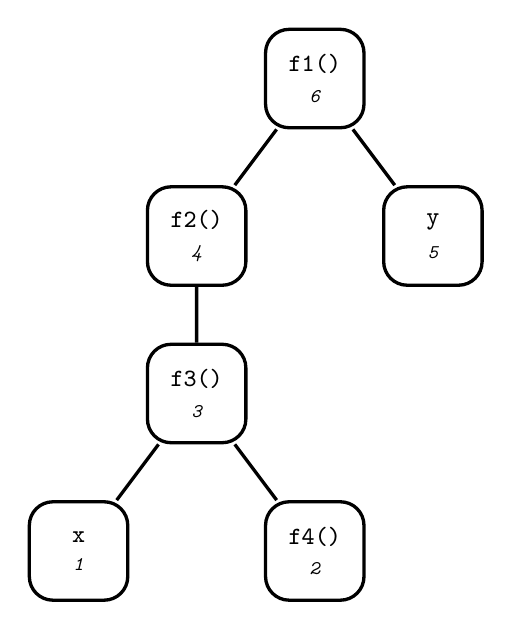
\begin{tikzpicture}[draw,very thick,font=\small\tt,
    rbx/.style={rectangle,draw,rounded corners=0.3cm,minimum size=1.25cm},
    level distance=2cm, sibling distance=3cm
]
  \tmpTree{4,7}
\end{tikzpicture}
\end{center}

The following figure shows the operations in forward execution order
with lines on the left side of the diagram showing the lifetime of
intermediate values. This represents the output of the liveness
analysis phase of the compiler. Because \texttt{f4} can be resumed by
\texttt{f1}, the value of the expression \texttt{x} has a lifetime
that extends to the invocation of \texttt{f1}. The extended portion of
the lifetime is indicated with a dotted line.

\begin{center}
\begin{tikzpicture}[draw,font=\small\tt, very thick]
%  \draw[help lines] (0,0) grid (16,5);
  \foreach \y in {4.2,3.4,2.6,1.8,1}
  {
    \draw (2,\y) -- ($ (1,\y) - 0.2*(\y ,0) + (0.84,0)$) -- ++(0,-0.8);
  }
  \node(x)[anchor=west]  at (2,4.2) {x};
  \draw ($ (x.west) - (1,1.6)$) -- ++(0,0.8);
  \draw[loosely dotted] ($ (x.west) - (1.0,1.7) $) -- (1,0.2);
  
  \node(f4)[anchor=west] at (2,3.4) {f4()};
  \node(f3)[anchor=west] at (2,2.6) {f3()};
  
  \node(f2)[anchor=west] at (2,1.8) {f2()};
  \draw ($ (f2.west) - (0.52,1.6)$) -- ++(0,0.8);
  
  \node(y)[anchor=west] at  (2,1.0) {y};
  \node(f1)[anchor=west] at (2,0.2) {f1()};
    
\end{tikzpicture}
\end{center}

The following series of diagrams illustrate the process of allocating
intermediate values. Each diagram includes an annotated syntax tree
and a status array for temporary variables. An arrow in the tree shows
the current location of the tree walk. A deallocation list is located
near the upper right of each node. An element in the list consists of
a temporary variable number and the status with which to restore the
variable's entry in the status array. If a temporary variable has been
allocated to an intermediate value, the variable's number appears near
the lower right of the corresponding node.

The status array is shown with four elements. The elements are
initialized to \textit{F} which indicates that the temporary variables
are free. A reserved temporary variable is indicated by placing the
node number of the reservation point in the corresponding
element. When a temporary variable is actually in use, the
corresponding element is set to \textit{I}.

Temporary variables are reserved while walking down the syntax
tree. The tree illustrated below on the left shows the state of
allocation after temporary variables have been allocated for the
operands of \texttt{f1}. Two contiguous variables are needed. All
variables are free, so the first-fit algorithm allocates variables 0
and 1. The status array is updated to indicate that these variables
are reserved for nodes \textit{4} and \textit{5} respectively, and the
nodes are annotated with these variable numbers. The lifetime
information in the previous figure indicates that these variables
should be deallocated after \texttt{f1} is executed, so the
deallocation array for node \textit{6} is updated.

The next step is the allocation of a temporary variable to the operand
of \texttt{f2}. The intermediate value has a lifetime extending from node
\textit{3} to node \textit{4}. This conflicts with the allocation of
variable 0, but not the allocation of variable 1. Therefore, variable
1 is allocated to node \textit{3} and the deallocation list for node
\textit{4} is updated. This is illustrated in the tree on the right:

\makebox[0.25in]{~}
\begin{tikzpicture}[draw,very thick,font=\small\tt,
    rbx/.style={rectangle,draw,rounded corners=0.3cm,minimum size=1.25cm},
    level distance=2cm, sibling distance=3cm
]
  \tmpTree{4,9}
  \stBox{3,1}{4}{5}{F}{F}
  % annotate the nodes
  \TR{f1}{\{0:\F, 1:\F\}};

  \TR{f2}{\{~\}};
  \BR{f2}{0};

  \TR{y}{\{~\}};
  \BR{y}{1};

  \TR{f3}{\{~\}};
  \TR{x}{\{~\}};
  \TR{f4}{\{~\}};

  \coordinate (arrow) at ($ (f1.north west) - (0.3,0.4)$);
  \draw[-Latex] (arrow) -- ($ (arrow) - (0,0.75)$);
\end{tikzpicture}
\makebox[0.75in]{~}
\begin{tikzpicture}[draw,very thick,font=\small\tt,
    rbx/.style={rectangle,draw,rounded corners=0.3cm,minimum size=1.25cm},
    level distance=2cm, sibling distance=3cm
]
  \tmpTree{4,9}
  \stBox{3,1}{4}{3}{F}{F}
  
  % annotate the nodes
  \TR{f1}{\{0:\F, 1:\F\}};

  \TR{f2}{\{1:{\sl 5\/}\}};
  \BR{f2}{0};

  \TR{y}{\{~\}};
  \BR{y}{1};

  \TR{f3}{\{~\}};
  \BR{f3}{1};
  \TR{x}{\{~\}};
  \TR{f4}{\{~\}};

  \coordinate (arrow) at ($ (f2.north west) - (0.3,0.4)$);
  \draw[-Latex] (arrow) -- ($ (arrow) - (0,0.75)$);
\end{tikzpicture}


The final allocation requires a contiguous pair of variables for nodes
\textit{1} and \textit{2}. The value from node \textit{1} has a
lifetime that extends to node \textit{6}, and the value from node
\textit{2} has a lifetime that extends to node \textit{3}. The current
allocations for variables 0 and 1 conflict with the lifetime of the
intermediate value of node \textit{1}, so the variables 2 and 3 are
used in this allocation. This is illustrated in the tree:

\begin{center}
\begin{tikzpicture}[draw,very thick,font=\small\tt,
    rbx/.style={rectangle,draw,rounded corners=0.3cm,minimum size=1.25cm},
    level distance=2cm, sibling distance=3cm
]
  \tmpTree{4,9}
  \stBox{3,1}{4}{3}{1}{2}

  % annotate the nodes
  \TR{f1}{\{0:\F, 1:\F, 2:\F\}};

  \TR{f2}{\{1:{\sl 5\/}\}};
  \BR{f2}{0};

  \TR{y}{\{~\}};
  \BR{y}{1};

  \TR{f3}{\{3:\F\}};
  \BR{f3}{1};

  \TR{x}{\{~\}};
  \BR{x}{2};
  
  \TR{f4}{\{~\}};
  \BR{f4}{3};
  
  \coordinate (arrow) at ($ (f3.north west) - (0.3,0.4)$);
  \draw[-Latex] (arrow) -- ($ (arrow) - (0,0.75)$);
\end{tikzpicture}
\end{center}


The remaining actions of the allocator in this example mark temporary
variables in-use when the code generator uses them and restore
previous allocated statuses when temporary variables are
deallocated. This is done in the six steps illustrated in the
following diagram. The annotations on the graph do not change. Only
the node of interest is shown for each step. These steps are performed
in node-number order.

\begin{center}
\begin{tikzpicture}[draw,very thick,font=\small\tt,
    rbx/.style={rectangle,draw,rounded corners=0.3cm,minimum size=1.25cm}
]
%  \draw[help lines] (0,0) grid (16,8);
  \node(x)[rbx] at (1,7) {\tmpLabel{x}{1}};
  \TR{x}{\{~\}};
  \BR{x}{2};
  \stBox{0,5}{4}{3}{I}{2}
  \draw[-Latex] ($ (x.south west) - (0.3, -0.2)$) -- ++(0,0.8);

  \node(f4)[rbx] at (6,7) {\tmpLabel{f4()}{2}};
  \TR{f4}{\{~\}};
  \BR{f4}{3};
  \stBox{5,5}{4}{3}{I}{I}
  \draw[-Latex] ($ (f4.south west) - (0.3, -0.2)$) -- ++(0,0.8);

  \node(f3)[rbx] at (11,7) {\tmpLabel{f3()}{3}};
  \TR{f3}{\{3:\F\}};
  \BR{f3}{1};
  \stBox{10,5}{4}{I}{I}{F}
  \draw[-Latex] ($ (f3.south west) - (0.3, -0.2)$) -- ++(0,0.8);

  \node(f2)[rbx] at (1,3) {\tmpLabel{f2}{4}};
  \TR{f2}{\{1:5\}};
  \BR{f2}{0};
  \stBox{0,1}{I}{5}{I}{F}
  \draw[-Latex] ($ (f2.south west) - (0.3, -0.2)$) -- ++(0,0.8);

  \node(y)[rbx] at (6,3) {\tmpLabel{y}{5}};
  \TR{y}{\{~\}};
  \BR{y}{1};
  \stBox{5,1}{I}{I}{I}{F}
  \draw[-Latex] ($ (y.south west) - (0.3, -0.2)$) -- ++(0,0.8);

  \node(f1)[rbx] at (11,3) {\tmpLabel{f1()}{6}};
  \TR{f1}{\{0:\F, 1:\F, 2:\F\}};
  \stBox{10,1}{F}{F}{F}{F}
  \draw[-Latex] ($ (f1.south west) - (0.3, -0.2)$) -- ++(0,0.8);

\end{tikzpicture}
\end{center}

In general, the tree walk will alternate up and down the syntax
tree. For example, if node \textit{5} had children, the allocation
status after the deallocation associated with node \textit{4},

\begin{center}
\begin{tikzpicture}[draw,very thick,font=\small\tt]
  \stBox{0,1}{I}{5}{I}{F}
\end{tikzpicture}
\end{center}

\noindent is used to allocate temporary variables to those
children. If this requires more than four temporary variables, the
status array is extended with elements initialized to \textit{F}.

This allocation algorithm is not guaranteed to produce an allocation
that uses a minimal number of temporary variables.  Indeed, a smaller
allocation for the previous example is illustrated in the tree:

\begin{center}
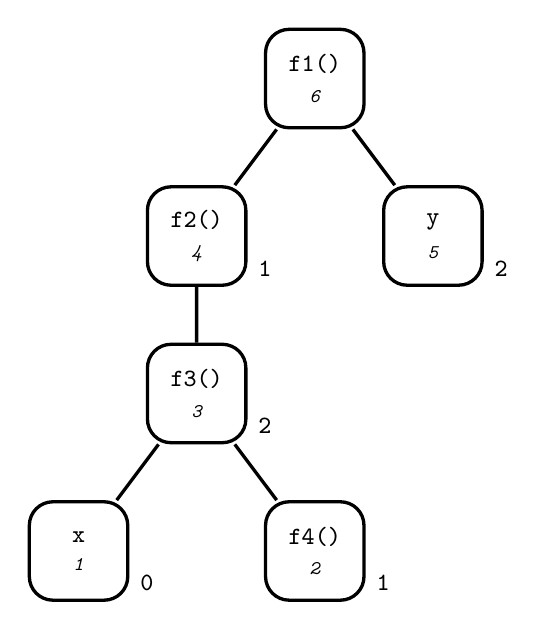
\begin{tikzpicture}[draw,very thick,font=\small\tt,
    rbx/.style={rectangle,draw,rounded corners=0.3cm,minimum size=1.25cm},
    level distance=2cm, sibling distance=3cm
]
  \tmpTree{4,9}

  % annotate the nodes
  \BR{f2}{1};
  \BR{y}{2};
  \BR{f3}{2};
  \BR{x}{0};
  \BR{f4}{1};
\end{tikzpicture}
\end{center}

While the non-optimality of this algorithm is unlikely to have a
measurable effect on the performance of any practical program, the
problem of finding an efficient optimal solution is of theoretical
interest. Classical results in the area of register allocation do not
apply. It is possible to allocate a minimum number of registers from
expression trees for conventional languages in polynomial time
[.dragon.]. The algorithm to do this depends on the fact that
registers (temporary variables) are dead as soon as the value they
contain is used. This is not true for Icon temporary variables.

The result of Prabhala and Sethi stating that register allocation is
NP-complete even in the presence of an infinite supply of registers
also does not apply [.prabhala subexp.]. Their complexity result
derives from performing register allocation in the presence of common
subexpression elimination (that is, from performing register
allocation on expression DAGS rather than trees) on a
2-address-instruction machine with optimality measured as the minimum
number of instructions needed to implement the program. Goal-directed
evaluation imposes more structure on lifetimes than common
subexpression elimination, the machine model used here is the C
language, and optimality is being measure as the minimum number of
temporary variables needed.

The Icon temporary variable allocation problem is different from the
Prolog variable allocation problem. Prolog uses explicit variables
whose lifetimes can have arbitrary overlaps even in the absence of
goal-directed evaluation. The Prolog allocation problem is equivalent
to the classical graph coloring problem which is NP-complete [.debray
apr91, dragon.].

If the allocation of a subarray of temporary variables is delayed
until the first one is actually needed in the generated code, an
optimum allocation results for the preceding example. It is not
obvious whether this is true for the general case of expression trees
employing goal-directed evaluation. This problem is left for future
work.

In addition to holding intermediate values, temporary variables are
used as local tended variables within in-line code.  This affects the
pattern of allocations, but not the underlying allocation technique.
